\section{Sanov's example and the family \texorpdfstring{$G_t$}{G\_t}}\label{sec:sanov}

For a real number $t$ let
\[
  A_t = \mat{1}{t}{0}{1}, \qquad B_t = \mat{1}{0}{t}{1}, \qquad
  G_t = \gen{A_t, B_t} \le \SL_2(\R).
\]
Sanov's matrices are $A = A_2$ and $B = B_2$. The group $G_t$ acts linearly on
$\R^2$, and for every integer $n$,
\[
  A_t^n(x,y) = (x + nty,\ y), \qquad B_t^n(x,y) = (x,\ ntx + y).
\]
So $A_t$ shears horizontally and $B_t$ vertically. We play ping-pong on the
two cones
\[
  X_1 = \{(x,y) : \abs{x} > \abs{y}\}, \qquad X_2 = \{(x,y) : \abs{y} > \abs{x}\},
\]
split by the sign of $xy$ into the four sets of Table~\ref{tab:sanov}.

\begin{table}[htbp]
  \centering
  \caption{Sanov's four sets. The last column states them as linear
  inequalities, without absolute values or products.}
  \label{tab:sanov}
  \begin{tabular}{@{}lll@{}}
    \toprule
    Set & Definition & As linear inequalities \\
    \midrule
    $D_A$      & $\abs{x} > \abs{y}$, $xy > 0$ & $x > y > 0$ or $x < y < 0$ \\
    $D_{A^{-1}}$ & $\abs{x} > \abs{y}$, $xy < 0$ & $x > -y > 0$ or $x < -y < 0$ \\
    $D_B$      & $\abs{y} > \abs{x}$, $xy > 0$ & $y > x > 0$ or $y < x < 0$ \\
    $D_{B^{-1}}$ & $\abs{y} > \abs{x}$, $xy < 0$ & $y > -x > 0$ or $y < -x < 0$ \\
    \bottomrule
  \end{tabular}
\end{table}

The case $t = 2$ of the next theorem is Sanov's~\cite{sanov-1947}, and the
general case is usually credited to Brenner~\cite{brenner-1955}. The proof is
the now-standard ping-pong argument; we have not compared it with the original
papers.

\begin{theorem}\label{thm:sanov}
If $t \in \R$ and $\abs{t} \ge 2$, then $A_t$ and $B_t$ freely generate a free
group of rank~$2$. In particular, Sanov's matrices $A$ and $B$ do.
\end{theorem}

\begin{proof}
Let $J = \mat{1}{0}{0}{-1}$. Then $J A_t J^{-1} = A_{-t}$ and
$J B_t J^{-1} = B_{-t}$, so replacing $t$ by $-t$ does not change the
question, and we may assume $t \ge 2$. We check the hypothesis
\eqref{eq:pingpong} of Theorem~\ref{thm:pingpong} for the sets of
Table~\ref{tab:sanov}, which are nonempty and pairwise disjoint.

Let $\varepsilon = \pm 1$. We show that $A_t^{\varepsilon}$ maps each of
$D_B$, $D_{B^{-1}}$ and $D_{A^{\varepsilon}}$ into $D_{A^{\varepsilon}}$.
Write $(x', y') = A_t^{\varepsilon}(x,y) = (x + \varepsilon t y,\ y)$.
\begin{itemize}
\item If $(x,y) \in D_B \cup D_{B^{-1}}$, then $\abs{y} > \abs{x}$, so
$t\abs{y} \ge 2\abs{y} > \abs{x}$. Hence $x'$ has the sign of
$\varepsilon t y$, and $\abs{x'} \ge t\abs{y} - \abs{x} > 2\abs{y} - \abs{y} = \abs{y}$.
So $\abs{x'} > \abs{y'}$, and $x'y' = x'y$ has the sign of
$\varepsilon t y^2$, which is the sign of $\varepsilon$.
\item If $(x,y) \in D_{A^{\varepsilon}}$, then $\varepsilon xy > 0$, so
$y \ne 0$ and $x$ has the same sign as $\varepsilon t y$. Hence
$\abs{x'} = \abs{x} + t\abs{y} > \abs{y}$, and
$x'y' = xy + \varepsilon t y^2$ has the sign of $\varepsilon$.
\end{itemize}
In both cases $(x', y') \in D_{A^{\varepsilon}}$. For $B_t$, let
$\sigma(x,y) = (y,x)$. Then $\sigma A_t \sigma = B_t$, and $\sigma$ carries
$D_{A^{\pm1}}$ to $D_{B^{\pm1}}$ and $D_{B^{\pm1}}$ to $D_{A^{\pm1}}$. So
$B_t^{\varepsilon}$ maps each of $D_A$, $D_{A^{-1}}$ and $D_{B^{\varepsilon}}$
into $D_{B^{\varepsilon}}$. Theorem~\ref{thm:pingpong} applies.
\end{proof}

\begin{figure}[htbp]
  \centering
  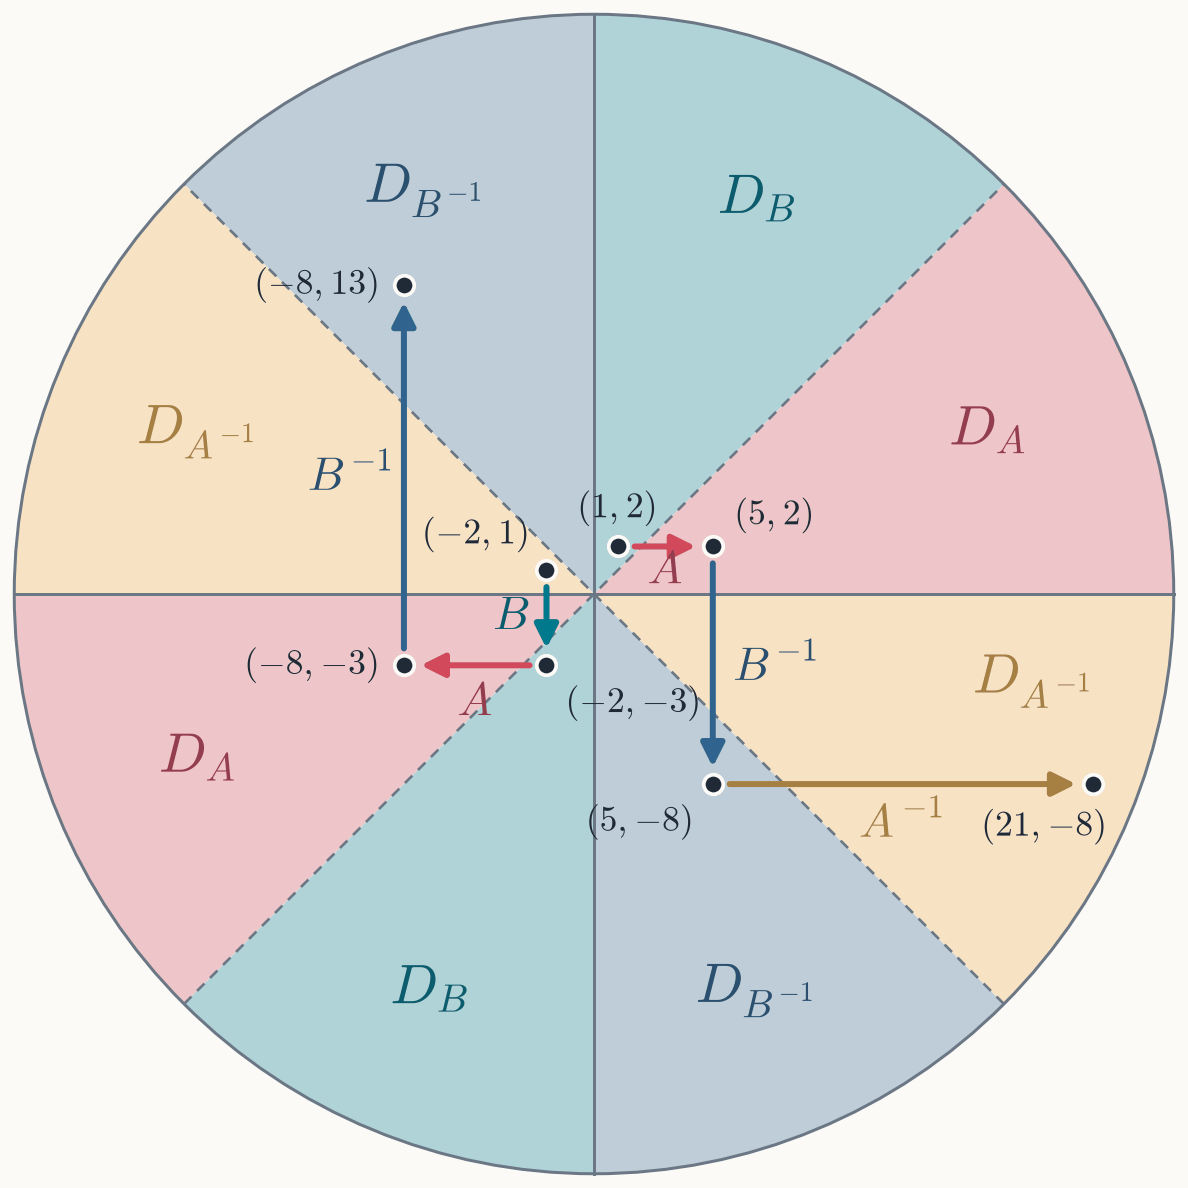
\includegraphics[width=0.48\linewidth]{cones.png}
  \caption{Sanov's sets for $t = 2$, and two short orbits starting at $(1,2)$
  and $(-2,1)$. Each arrow applies one letter, and the point lands in the set
  of that letter, as in the proof of Theorem~\ref{thm:pingpong}. The axes and
  the diagonals lie in none of the four sets.}
  \label{fig:cones}
\end{figure}

Figure~\ref{fig:cones} shows the sets for $t = 2$. The orbit of $(1,2)$, for
example, reads
\[
  (1,2) \xrightarrow{\;A\;} (5,2) \xrightarrow{\;B^{-1}\;} (5,-8)
  \xrightarrow{\;A^{-1}\;} (21,-8),
\]
so the word $A^{-1}B^{-1}A$ moves $(1,2) \in D_B$ into $D_{A^{-1}}$.

\begin{remark}\label{rem:two-cones}
Sanov's argument is often stated with the two cones and
Theorem~\ref{thm:tabletennis}. If $n \ne 0$ and $(x,y) \in X_2$, then
$\abs{x + nty} \ge \abs{n}\abs{t}\abs{y} - \abs{x} > 2\abs{y} - \abs{y} = \abs{y}$,
so $A_t^n(X_2) \subseteq X_1$. Likewise $B_t^n(X_1) \subseteq X_2$. Since
$A_t$ and $B_t$ have infinite order, Example~\ref{ex:freeproduct} gives
$G_t \cong \Z * \Z$.
\end{remark}

\begin{remark}\label{rem:schottky-fails}
The Schottky hypothesis of Remark~\ref{rem:variants} fails here: $A$ fixes
$(1,0)$, which lies outside $D_{A^{-1}}$ but not in $D_A$. This is why we use
the weaker hypothesis \eqref{eq:pingpong}. Since the sets are cones, the
argument also runs on the projective line $\RP^1$. In terms of the slope
$m = y/x$, the four sets become the intervals
\[
  D_A = (0,1), \quad D_{A^{-1}} = (-1,0), \quad D_B = (1,\infty), \quad
  D_{B^{-1}} = (-\infty,-1).
\]
Their closures touch at the slopes $0$, $\pm1$ and $\infty$. On slopes, $A$
acts by $m \mapsto m/(1+2m)$, a parabolic map whose only fixed point is the
point $0$ where $D_A$ and $D_{A^{-1}}$ meet. So the picture is like that of a
Schottky group (Section~\ref{sec:schottky}), except that the intervals touch
and the generators are parabolic.
\end{remark}

\subsection{The non-example \texorpdfstring{$t = 1$}{t = 1}}
At $t = 1$ the argument must fail, because $G_1$ is not free:
\[
  A_1 B_1^{-1} A_1 = \mat{1}{1}{0}{1} \mat{1}{0}{-1}{1} \mat{1}{1}{0}{1}
  = \mat{0}{1}{-1}{0}
\]
has order $4$. So the nonempty reduced word
\[
  (a b^{-1} a)^4 = a b^{-1} a^2 b^{-1} a^2 b^{-1} a^2 b^{-1} a
\]
is equal to $1$ in $G_1$ when $a = A_1$ and $b = B_1$. In fact $G_1 = \SL_2(\Z)$, by the classical fact that these two
elementary matrices generate $\SL_2(\Z)$. The cones fail, as they must:
$A_1(-1,2) = (1,2)$, so $A_1$ does not map $X_2$ into $X_1$. The same happens
for every $t$ with $0 < \abs{t} < 2$, since $A_t(-t/2, 1) = (t/2, 1)$ stays in
$X_2$. For such $t$ the cones say nothing, and other methods are needed;
Section~\ref{sec:open} describes what is known when $t^2$ is rational.
